\documentclass[border=5mm]{standalone}
\usepackage{luamplib}
\usepackage{graphicx}
\mplibtextextlabel{enable}
\begin{document}

    \begin{mplibcode}

beginfig(0);
    picture A,B;
    A = TEX("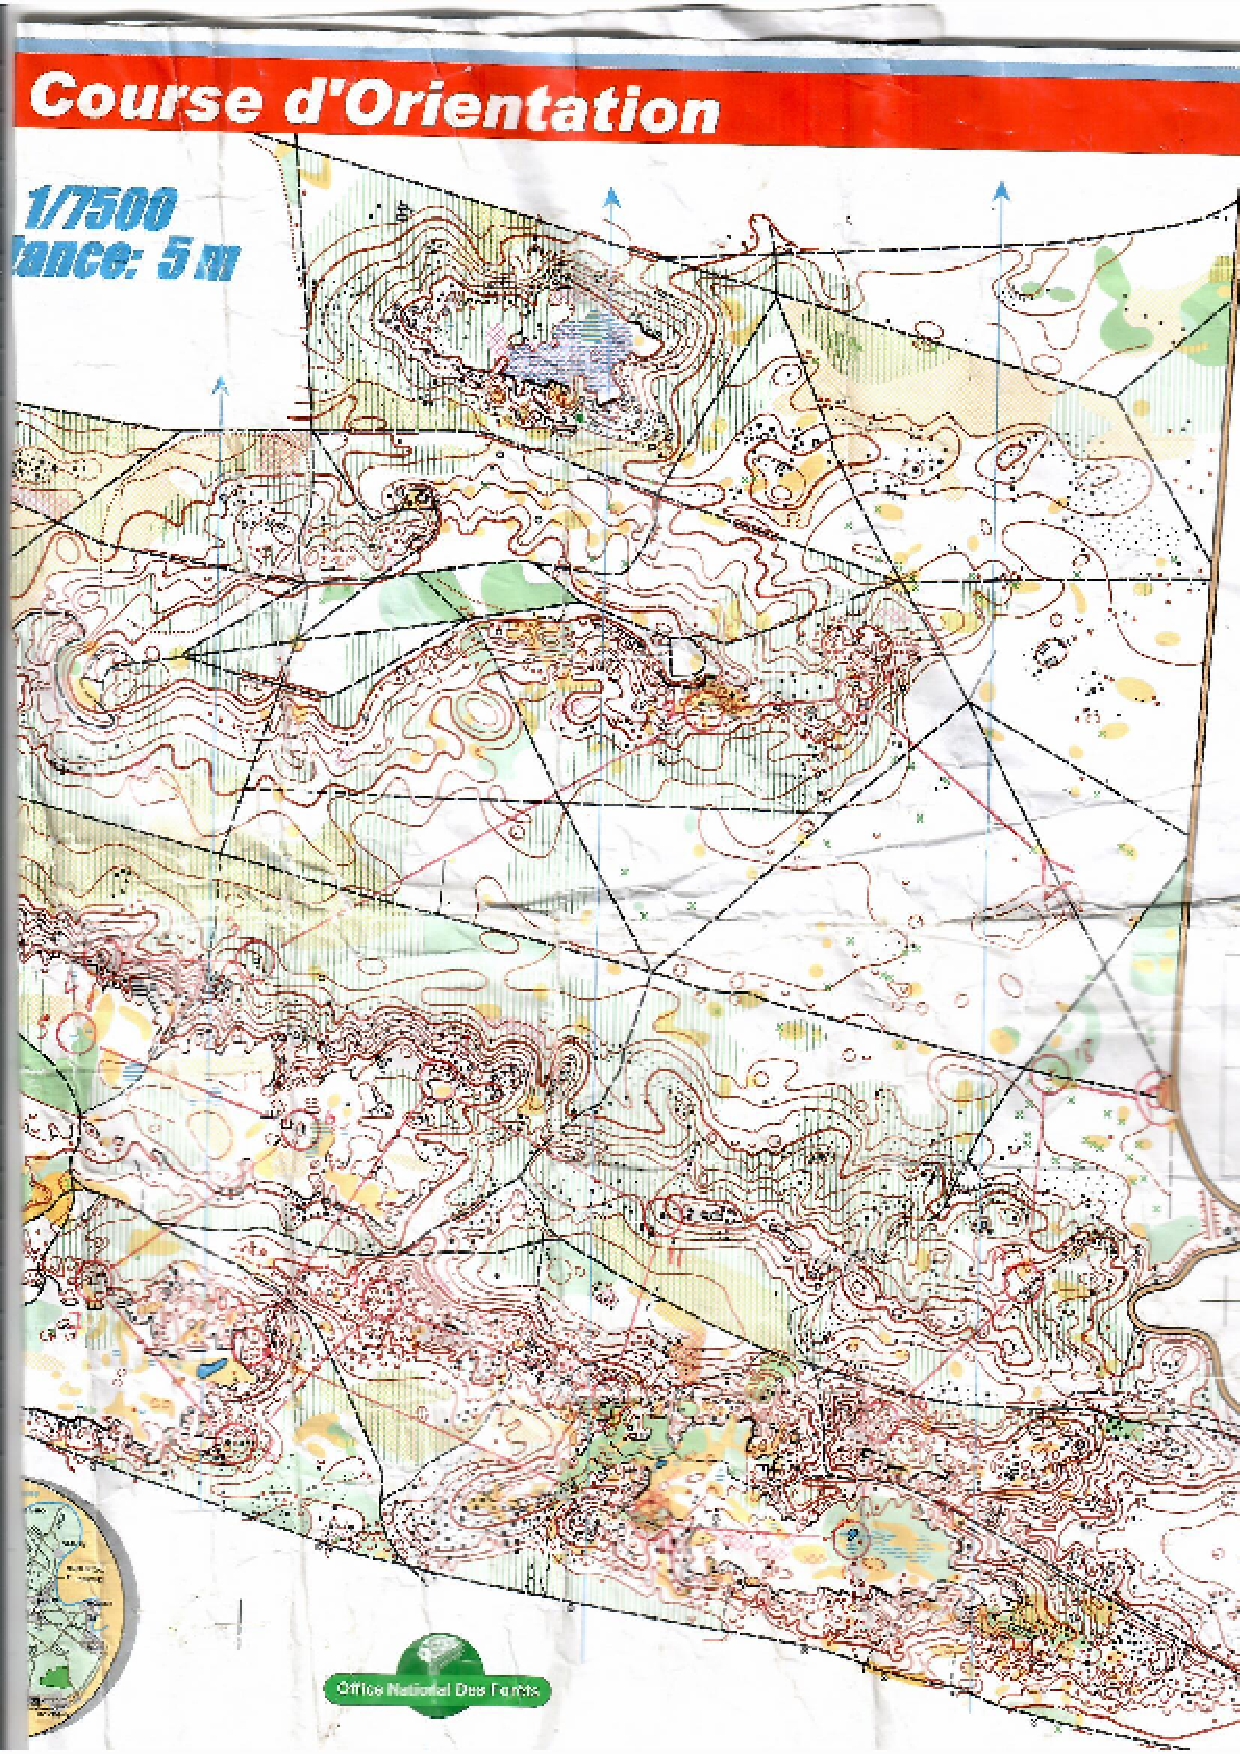
\includegraphics[width=300pt]{le-carrosse.pdf}");
%    B = TEX("\includegraphics[width=300pt]{marly.mps}");

    xmin=3 ;
    xmax=10 ;
    ymin = 1.1 ;
    ymax = 10 ;



    draw A ;



    pair X ;
    X:=(282,160) ;
    %fill fullcircle scaled 5 shifted X withcolor (1,0,0) ;


    numeric dx,dy,ratio,theta ;
    dx=-10;
    dy=75 ;
    ratio=1 ;
    theta=0 ;
    %draw B  scaled ratio shifted X rotated theta ;

    %path b ;
    %b = bbox B ;
    %draw b withcolor (1,0,0) ;


endfig;

\end{mplibcode}

\end{document}
